\Problem{Dirty Driving}{driving}
% author: Jon Marius Venstad

\begin{wrapfigure}{r}{7cm}
\vspace{-5mm}
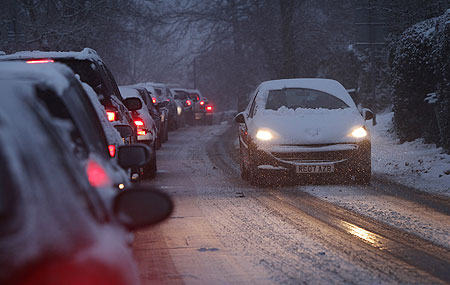
\includegraphics[width=\linewidth,keepaspectratio=true]{driving/driving}
\vspace{-9mm}
\end{wrapfigure}

\noindent
Like all other good drivers, you like to curse, swear and honk your horn at your fellow automobile drivers. Today you're at the rear of a long line, brooding over the others' inability to keep proper distance to the car in front. But are you really keeping your own distance?

You have calculated that in order to never have to use your breaks, you must keep a distance to any car $x$ in front of you at least $p(n+1)$ where $n$ is the number of cars between you and $x$, and $p$ is an integer constant determined by which of your cars you are currently driving. 

Given the value of $p$ and the current distances (in random order) to each of the cars ahead of you, calculate the minimum distance you \textit{should} be keeping to the car directly in front, in order to not have to use your breaks.

\Input
A line with $1 \leq n \leq 100000$ -- the number of cars ahead of you -- and $1 \leq p \leq 20$ -- the deceleration constant.\\
A single line with $n$ unique integers denoting the current distance to each of the cars ahead of you. Each of these integers are in the interval $[1, 10^7]$\\

\Output
The minimum distance you must keep to the car directly in front, in order to not have to use your breaks.\\

\Xample{driving/driving.1}

\Xample{driving/driving.2}
